% ----------------------------------------------------------
% Protocolos de comunicaçào
% ----------------------------------------------------------
\chapter[Estudo de Caso]{Estudo de Caso}
%\addcontentsline{toc}{chapter}{Protocolos de Comunicação}
% ----------------------------------------------------------

Para obter um exemplo do mundo real, o estudo de caso foi projetado com base em uma aplicação de WMS (\textit{Warehouse Management System}). \citeonline{wms-definition} explica que um sistema de WMS é um software que auxilia as operações do dia-a-dia em um armazém. Os sistemas WMS permitem o gerenciamento centralizado de tarefas, como o rastreamento de níveis de inventário e locais de estoque. Os sistemas WMS podem ser  um aplicativo independente ou parte de um sistema de ERP.

Com o intuito de realizar consultas relevantes, foi modelado um esquema contendo seis entidades, capazes de representar consultas reais, e ainda produzirem informações pertinentes para a comparação de desempenho. A construção das APIs seguiram os princípios do ciclo tradicional do desenvolvimento de software, portanto a modelagem foi elaborada antes do início da implementação das APIs. Isso assegura que nenhuma decisão de tecnologia afetou a modelagem das entidades, que pode ser exemplificado na figura \ref{fig:marlon}.

\begin{figure}[htbp]
\centering
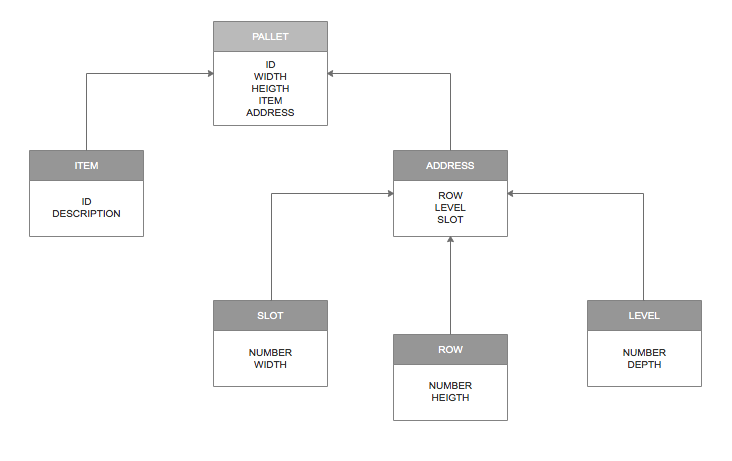
\includegraphics[width=0.9\textwidth]{figuras/model.png}
\caption{Modelagem WMS}
\label{fig:marlon}
\author{fonte: Autor}
\end{figure}

A modelagem acima, representa o gerenciamento de um armazém, com capacidade de armazenar diversos itens. Os itens são dispostos em pallets, e alocados em endereços dentro do armazém. Como pode ser observado na figura \ref{fig:rack}, os endereços do armazém são formados a partir de uma combinação de três \textit{dimensões}: Prateleira, Linha e Nível. Cada combinação dessas três propriedades é capaz de alocar um pallet, que por sua vez pode conter diversas unidades de um mesmo item.

Imagine um item de código 22B12, por exemplo, que representa um produto X. Este produto é disposto em um pallet com capacidade de armazenar 30 unidades do item 22B12. O armazém é composto por 26 prateleiras, sequenciadas de 'A' a 'Z'. Cada prateleira possui 2 linhas de profundidade e  3 níveis de altura. O pallet com o código 001 contém 30 unidade do item 22B12, e precisa ser alocado dentro armazém, para isso é utilizado um sistema de códigos envolvendo as 3 dimensões do armazém.


\begin{figure}[htbp]
\centering
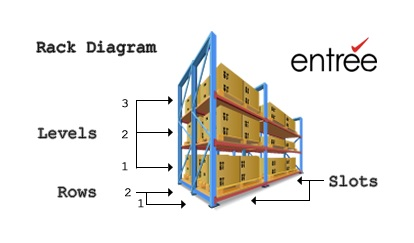
\includegraphics[width=0.7\textwidth]{figuras/rack.jpg}
\caption{Diagrama de dimensões do armazém (REFAZER)}
\label{fig:rack}
\author{fonte: Autor}
\end{figure}

60 unidades do item 22B12 estão dispostos em dois pallets(001, 002) existentes no armazém e cada um dos pallets será destinado a um endereço. O pallet 001 será alocado na terceira prateleira, no segundo nível e na primeira linha. Após a formação do endereço, o pallet 001 estará localizado no endereço C0101.  

\section{Hipóteses} \label{sechHipóteses}

Hipóteses na diferença de desempenho entre as APIs derivaram dos fundamentos teóricos. Elas baseiam-se no entendimento de que os protocolos utilizados possibilitam a implementação de uma combinação de técnicas afim de afetar positivamento o desempenho da API. Portanto, ambas as implementações devem ter as mesmas propriedades, seguindo suas melhores práticas, modelos de maturidade e documentação.

As hipóteses deste trabalho são: 

\begin{itemize}
\item Utilizando GraphQL irá reduzir o tamanho da resposta;
\item Utilizando GraphQL irá reduzir o tempo de resposta;
\item Utilizando REST irá reduzir a utilização de consumo de CPU;
\item Utilizando REST irá reduzir o consumo de Memória;
\end{itemize}

Com o propósito de validar as hipóteses definidas, foram determinadas duas perguntas que envolvessem todas as entidades. Para cada pergunta existe apenas uma resposta correta e sua lógica é baseada em campos das estruturas de dados de retorno.

\textbf{Questão 1}: Qual item ocupa a maior quantidade de pallets alocados no armazém?

\textbf{Questão 2}: O item 22B12 está armazenado em quais endereços?

\section{Cenários} \label{sec:cenarios}

A escolha das ferramentas a serem usadas na implementação foi uma das partes mais importantes no planejamento do estudo de caso. Foi necessário pensar em uma especificação que apresentasse uma curva rápida de aprendizagem, um fluxo de execução replicável e agnóstico à plataforma, e uma documentação madura em relação a implementação das APIs.

As APIs foram escritas na linguagem de programação JavaScript, utilizando a especificação do ECMAScript 5. Foi escolhido esta linguagem com vista ao fácil acesso a bons frameworks para construção de serviços WEB, como o Node.js. Node.js é uma plataforma para desenvolvimento de servidores web baseadas em rede utilizando JavaScript e o V8 JavaScript Engine, ou seja, com Node.js pode-se criar uma variedade de aplicações Web utilizando código em JavaScript \citeonline{node-definition}.

\subsection{Ferramentas utilizadas}

Node.js dispõe de inúmeros recursos e ferramentas que possibilitam a construção de APIs. Mesmo assim, o ecosistema de bibliotecas no Node.js conta com ferramentas que simplificam ainda mais a construção de aplicações para servidores Web. Nesta sessão serão citados algumas nessas bibliotecas que foram utilizadas para desenvolver tanto a API REST quando a API GraphQL. 

\subsubsection*{Expess.JS}

Express é um \textit{framework} para Node.js extremamente flexível, que forcene um conjunto robusto de feramentas para a construção de aplicações Web e Móveis. Conta com um robusto sistema de roteamento, facilitando o desenvolvimento de APIs. O Express forcene uma fina camada de abstração nas principais funcionalidades do Node.js, sem sobrepor os recursos no Node.

Nos protótipos desenvolvidos para executar o experimento, o Express teve como papel de \textit{middleware} gerenciando as rotas, e delegando a resposabilidade de interpretação das requisições para os \textit{Controllers} na API REST e para os \textit{Resolvers} na API GraphQL.

O código \ref{lst:load-rest} ilustra como os \textit{Controllers} enviam as informações da requisição para o model, que é o responsável na API REST em executar as consultas no banco de dados. No exemplo abaixo, o trexo de código é o responsavel por retornar um Item baseado no id recebido como parâmetro da requisição.

\begin{lstlisting}[escapeinside={(*}{*)}, numbers=left, caption={Controller para carregar um item}, label=lst:load-rest,language=Java]
//item.controller.js
import Item from '../models/item.model';

/**
 * Load item and append to req.
 */
function load(req, res, next, id) {
  Item.get(id)
    .then((item) => {
      req.item = item;
      return next();
    })
    .finally(e => next(e));
}

\end{lstlisting}

Já o código \ref{lst:express-graph} mostra como o Express.JS gerencia a requisição recebida via método GET, e delega a responsabilidade para o schema.js, onde esta contido a lógica para a interpretação dos parâmetros da requisição e retornar um objeto JSON com a devida resposta.

\begin{lstlisting}[escapeinside={(*}{*)}, numbers=left, caption={Controller para carregar um item}, label=lst:express-graph,language=JavaScript]
//server.js
import express from 'express';
let app = express();

import schema from './schema.js';

app.get('/', (req, res) => {
    graphql(schema, req.query.query)
    .then((result) => {
        res.send(result);
    });
});

\end{lstlisting}

\subsubsection*{MongoDB}

MongoDB é um banco de dados \textit{open source} que utilizada um modelo de dados orientado a objetos. O mesmo tem como característica conter todas as informações importantes em um único documento, possuir identificadores únicos universais (UUID), possibilitar a consulta de documentos através de métodos avançados de agrupamento e filtragem, também conhecido como \textit{MapReducers}. Ao invés de usar tabelas e linhas, como os bancos de dados relacionais, o MongoDB usa uma arquitetura baseada em coleções e documentos.


\subsubsection*{Ferrametas clientes}

Serão utilizadas ferramentas que se comportaram como cliente das APIs construídas. O foco deste trabalho não é em cima das aplicação clientes, entretanto é importante conhece-las pois são elas que invocarão as consultas como também é através delas que algumas métricas serão extraidas. O software Postman será usado fundamentalmente para a execução das buscas nas APIs.

O Postman é uma cadeia completa de ferramentas para desenvolvedores de APIs, usadas empresas em todo o mundo. O Postman é uma ferramenta elegante e flexível usada para construir softwares conectados via APIs - de forma rápida, fácil e precisa. Fundada em 2014, a empresa escalou grandes alturas e hoje, ela é utilizada por mais de 3 milhões usuários ao redor do mundo.

Ele funciona como uma emulador para execução de consultas em APIs. Com ele é possível executar buscas utilizando qualquer dos métodos do protocolo HTTP, possibilitando customizaçào tando do corpo quando do cabaçario das requisições se preciso. Junto com a resposta da consulta, o Postman traz também informações extremamente relevantes, como tempo que a API levou para responder e o tamanho em bytes contido na resposta. Essas funcionalidade alidas com a opção de executar um numero customizavel de iterações para cada requisição, será a base para avaliar o desempenho das APIs REST e GraphQL.

\subsection{Ambiente}

A configuração da máquina utilizada para o teste de desempenho local é descrita na Tabela \ref{tab:host}. As APIs REST e GraphQL foram construídas para responder as requisições recebidas retornando respostas no formato JSON, a fim de gerar um fator de medição de desempenho da execução dos testes. Para a execução do experimento, apenas os softwares necessários estavam ativos, portanto, ao executar as buscas, o servidor REST ou GraphQL estará ativo, além do servidor de banco, as aplicações clientes, e as aplicações de coleta das métricas.

\begin{table}
    \centering
    \begin{tabular}{| l | l |}
        \hline
        \textbf{Item} & \textbf{Descrição} \\ \hline
        Marca/Modelo & Mac \\ \hline
        Processador & Intel \\ \hline
        Memória &  X GB  \\ \hline
        Disco rígido & SSD 128  \\ \hline
        Quantidade núcleos & 4  \\ \hline
    \end{tabular}
    \caption{Configuração do Ambiente} \label{tab:host}
\end{table}

\subsection{Detalhes implementação REST}

O servidor REST consiste em um servidor HTTP escrito em Node.js que recebe as requisições HTTP recebidas. Dependendo do método e URL da requisição, rooteia-o para o \textit{controller} correspondente. O \textit{controller} faz a consulta na base de dados do MongoDB. Ao realizar o gerenciamento das rotas, o servidor realiza os devidos logs de latência . Após a consulta, a resposta desejada é enviada de volta para o cliente. Esse fluxo acontece em qualquer cenário, independente do número de requisições desejadas.

No presente trabalho, como o objetivo é apenas medir o desempenho de consultas utilizando REST, todas as requisições utilizarão o método HTTP GET. Para as medições da API REST, a aplicação cliente irá enviar por exemplo, uma requisição para recuperar todos os itens cadastrados. Como pode ser observado da tabela \ref{tab:rest-url}, é necessário executar uma busca do tipo localhost:8080/item, que que irá ser interpretada pelo servidor REST, identificando qual é a rota responsável por essa requisição. A servidor consultará a base de dados retornando uma resposta no formato JSON, com todos os itens cadastrados na API. Esse fluxo é ilustrado na figura \ref{fig:rest-uml}

\begin{table}
    \centering
    \begin{tabular}{| l | l |}
        \hline
        \textbf{URI} & \textbf{Descrição} \\ \hline
        /item & Consulta lista de itens \\ \hline
        /item/:id & Consulta item pelo id \\ \hline
        /pallet & Consulta lista de pallets  \\ \hline
        /pallet/:id & Consulta pallet pelo id  \\ \hline
        /address & Consulta lista de endereços \\ \hline
        /address/:id & Consulta endereço pelo id \\ \hline
        /slot & Consulta lista de prateleiras \\ \hline
        /slot/:id & Consulta prateleira pelo id \\ \hline
        /row & Consulta lista de linhas \\ \hline
        /row/:id & Consulta linha pelo id \\ \hline
        /level & Consulta lista de nível \\ \hline
        /level/:id & Consulta nível pelo id \\ \hline
    \end{tabular}
    \caption{Servidor REST} \label{tab:rest-url}
\end{table}

\begin{figure}[htbp]
\centering
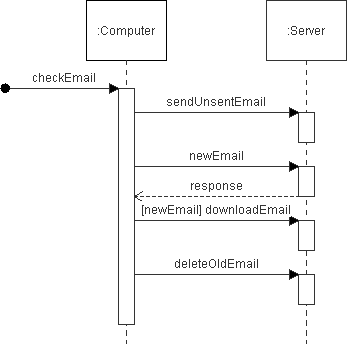
\includegraphics[width=0.5\textwidth]{figuras/uml-sequence.png}
\caption{UML sequence REST (REFAZER)}
\label{fig:rest-uml}
\author{fonte: Autor}
\end{figure}
\pagebreak

\subsection{Detalhes implementação GraphQL}

O servidor GraphQL foi implementado também usando Node.js. A diferença em comparação com a implementação do servidor REST é que o servidor GraphQL envia todos os pedidos ao núcleo GraphQL ao invés de rotear as requisições recebidas para vários \textit{controllers} diferentes. O GraphQL analisa a consulta e envia os parâmetros para os \textit{resolvers} responsáveis, localizados nos \textit{schemas} GraphQL. \textit{Rsolvers} são funções definidas para todos os campos no \textit{schema} GraphQL, cada um retorna os dados para o campo específico. Estas funções são executadas quando os campos correspondentes são consultados e os resultados são retornados na resposta.

\begin{lstlisting}[escapeinside={(*}{*)}, numbers=left, caption=Consulta de itens]
query RootQuery {
	items {
    	id
    	description
    }
}

\end{lstlisting}

 \textit{ A consulta acima retorna como resposta lista a de todos os itens cadastrados na base de dados. Note que a resposta contém apenas os atributos que a consulta requisitou: }

\begin{lstlisting}[escapeinside={(*}{*)}, numbers=left, caption=Listagem dos itens (Validar)]
{
    "data": [
         {
        	"id": 22B12
            "description": "Flat screen",
        },
        {
        	"id": 21C44
            "description": "Computer screen",
        },
        {
        	"id": 43F12
            "description": "Smartphone screen",
        },
    ]
}

\end{lstlisting}

Aqui tenho que explicar o diagrama de sequência para o GraphQL

\begin{figure}[htbp]
\centering
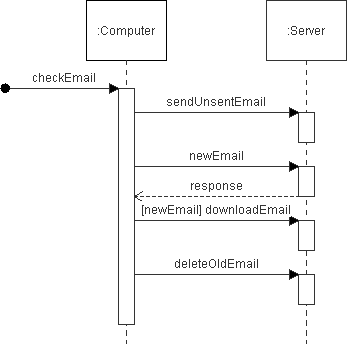
\includegraphics[width=0.5\textwidth]{figuras/uml-sequence.png}
\caption{UML sequence GraphQL (REFAZER)}
\label{fig:graph-uml}
\author{fonte: Autor}
\end{figure}
\pagebreak


\section{Métricas}\label{sec:metrics}

Afim de comparar as medidas de desempenho de APIs desenvolvidas em REST com APIs desenvolvidas em GraphQL, algumas métricas precisam ser definidas. O desempenho de cada API vai depender de sua implementação, porém, escolhendo as métricas corretas, o efeito da implementação pode ser reduzido. Focando em medições corretas, as diferenças relevantes das APIs podem ser destacadas e melhor ponderadas.

Para o presente trabalho, serão utilizadas quatro métricas diferentes: Utilização da CPU, Consumo de memória, Tempo de resposta e o Tamanho da resposta. É importante ressaltar que cada métrica foi medida separadamente, para que \textit{logs} e \textit{outputs} pertinentes a uma métrica específica não interfira no resultado das demais.

\subsection*{Utilização da CPU}

A utilização da CPU é uma medida do percentual de ciclos que representa uma porcentagem em que as unidades de processamento ficam dedicadas a executar um processo em particular. No contexto do presente trabalho, é a porcentagem de processamento dentro da CPU utilizada em cada requisição.

Esta métrica será extraída atraves do módulo \textit{OS} presente no \textrm{core} do Node.Js. A função \textit{os.loadavg()} trás como resultado uma medida da atividade do sistema, calculada pelo sistema operacional e expressa como um número fracionário. A média será a medida de comparação entre as duas abordagens. A seguinte fórmula será usada para calcular esta métrica: 

$$S=mrs1+mrz2..+mrsn$$

Onde $MRS$ é o tempo total para obtido em cada requisição necessária, e $S$ representa a soma dos tempos, resultando do 

\subsection*{Consumo de memória}

O consumo de memória, junto com a utilização da CPU, é uma das medidas mais importantes pois é nesses pontos que observamos o verdadeiro custo por trás da escolha da ferramenta. O consumo de memória é a quantidade de em bytes utilizado pela API, e será medido através da soma da utilização de memória em cada consulta necessária para atender os senários propostos. A seguinte fórmula será usada para calcular esta métrica: 

$$S=mrs1+mrz2..+mrsn$$

Onde $MRS$ é o tempo total para obtido em cada requisição necessária, e $S$ representa a soma dos tempos, resultando do 

Ferramenta X utilizada

\subsection*{Tempo de resposta}

Tempo que cada requisição levou para realizar a consulta. Esse tempo é calculado a partir do início da requisição, até o retorno da resposta completa. No caso da API REST, esta métrica será acumulativa, ou seja, a soma do tempo de todas as requisições necessárias. A seguinte fórmula será usada para calcular esta métrica: 

$$S=mrs1+mrz2..+mrsn$$

Onde $MRS$ é o tempo total para obtido em cada requisição necessária, e $S$ representa a soma dos tempos, resultando do 

\subsection*{Tamanho da resposta}

O tamanho da resposta será calculada baseado no tamanho em textit{bytes} da resposta. Essa métrica será calcula a partir da média de 12 consultas. Novamente, para a API REST será usada a média das somas de todas as consultas necessárias para obter a resposta desejada. A seguinte fórmula será usada para calcular esta métrica: 

$$S=mrs1+mrz2..+mrsn$$

Onde $MRS$ é o tempo total para obtido em cada requisição necessária, e $S$ representa a soma dos tempos, resultando do 

\subsection*{Conclusão}

\begin{figure}[htbp]
\centering
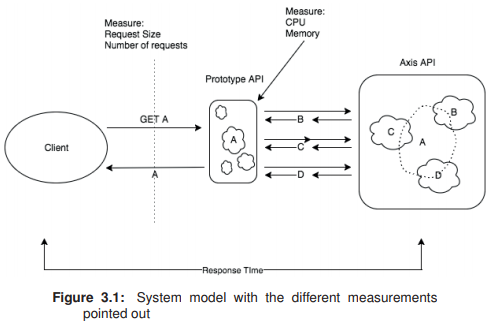
\includegraphics[width=0.8\textwidth]{figuras/metricas.PNG}
\caption{Arquitetura das APIs e diferentes pontos de medidas (REFAZER)}
\label{fig:my-metrics}
\author{fonte: Autor}
\end{figure}

A figura \ref{fig:my-metrics} mostra como as métricas serão extraidas. A utlização do CPU e o consumo de memória serão medida utilizando ferramentas do próprio Node.js. Ambos serão medidos via \textit{logs} no código fonte dos protótipos implementados. O tamanho da resposta e o tempo de resposta serão extraídos utilizando a ferramenta Postman, ao final de cada consulta.